%==============================================================================
% GradeAI -- first_draft.tex  (SKELETON)
% CSC398H5 F (Fall 2026) -- Red Hat x IBM InstructLab
% Final paper due: December 7, 2026
%
% HOW TO USE THIS FILE
%   * \todo{Owner}{what to do}   -> red inline note. Search for "\todo" to find work.
%   * \ph{...}                   -> BLUE text = placeholder/target number that is
%                                   NOT a real result yet. Replace with cluster output
%                                   and remove the \ph{} wrapper.
%   * % TODO [Owner]: ...        -> source-code comment pointing at the log/file to use.
%   * Before submission: set \draftfalse below to hide all todos and colouring.
%==============================================================================
\documentclass[11pt,a4paper]{article}

%---------------------------- Packages ----------------------------------------
\usepackage[utf8]{inputenc}
\usepackage[T1]{fontenc}
\usepackage[margin=1in]{geometry}
\usepackage{microtype}
\usepackage{amsmath,amssymb,amsfonts,amsthm}
\usepackage{booktabs}
\usepackage{graphicx}
\usepackage{xcolor}
\usepackage{tikz}
\usetikzlibrary{arrows.meta,positioning,shapes.geometric,fit}
\usepackage{listings}
\usepackage{enumitem}
\usepackage{tabularx}
\usepackage{caption}
\usepackage[colorlinks=true,linkcolor=blue!50!black,citecolor=blue!50!black,urlcolor=blue!50!black]{hyperref}
\usepackage[capitalise,noabbrev]{cleveref}

%---------------------------- Draft helpers -----------------------------------
\newif\ifdraft
\drafttrue   % <-- change to \draftfalse for the final version

\newcommand{\todo}[2]{%
  \ifdraft\textcolor{red}{\textbf{[TODO #1:} #2\textbf{]}}\fi}
\newcommand{\ph}[1]{\ifdraft\textcolor{blue!70!black}{#1}\else #1\fi}

%---------------------------- Listings style ----------------------------------
\lstdefinestyle{prompt}{
  basicstyle=\ttfamily\footnotesize,
  breaklines=true, breakatwhitespace=true,
  frame=single, rulecolor=\color{black!30},
  backgroundcolor=\color{black!3},
  columns=fullflexible, keepspaces=true,
  xleftmargin=0.5em, xrightmargin=0.5em, aboveskip=1em, belowskip=1em
}
\lstset{style=prompt}

%---------------------------- Macros ------------------------------------------
\newcommand{\gradeai}{\textsc{GradeAI}}
\newcommand{\indic}{\mathbb{I}}
\newcommand{\levels}{\mathcal{L}}
\DeclareMathOperator*{\argmax}{arg\,max}
\theoremstyle{definition}
\newtheorem{definition}{Definition}

%---------------------------- Title -------------------------------------------
\title{\textbf{\gradeai: Synthetic Data Generation, InstructLab, and Open-Weights LLMs for Privacy-Preserving Automated Proof Grading and Uncertainty-Aware Triage (blah) }\\[0.6em]
\large CSC398H5: Topics in Computer Science --- Building Ethical Software Solutions
with Industry Collaboration (Red Hat $\times$ IBM InstructLab, Fall 2026)}


\author{%
  Name 1 \and Name 2 \and Name 3 \and Name 4 \and Name 5\\[0.5em]
  University of Toronto Mississauga\\
  Department of Mathematical and Computational Sciences
  % TODO [All]: Add emails / roles if required by the instructor.
}
\date{December 7, 2026}

\begin{document}
\maketitle

%==============================================================================
\begin{abstract}
% TODO [Name 1 - Writing Lead]: Rewrite once results are final; target <= 250 words.
% Structure: Problem -> Gap -> Approach -> Results -> Privacy/ethics.
\todo{}{title}

\todo{}{Reorient abstract to InstructLab and SDG and related concepts rather than GradeAI}
Grading undergraduate mathematical proofs in courses such as CSC236 and MAT102 is slow, inconsistent across teaching assistants (TAs), and subject to privacy constraints that prohibit sending student work to commercial LLM APIs. Zero-shot LLMs [note: that is, prompting a pretrained LLM without context] are a poor substitute: they tend to \todo{}{problem 1} and their grades are unstable under rewording. 
We present \gradeai{}, a human-in-the-loop grading assistant created by fine-tuning an open-weights model with InstructLab-generated synthetic data and LoRA. The model outputs only per-criterion rubric levels with short justifications; point totals are computed deterministically in software.
Confidence is estimated by \todo{}{Estimate confidence}, and submissions with low agreement or malformed output are routed to \todo{}{Where} for mandatory review. On a locked benchmark of \ph{\todo{}{X}} synthetic proofs, \gradeai{} reaches \ph{\todo{}{X}\%} per-criterion agreement with human consensus (X), keeps grades invariant on \ph{X\%} of rewordings, and concentrates errors in the \ph{X\%} of submissions it flags for review.

\end{abstract}

\noindent\textbf{Keywords:} automated grading, mathematical proofs, InstructLab, LoRA, selective classification, privacy, human-in-the-loop, educational ethics. \todo{}{Add or remove keywords}

%==============================================================================
\section{Introduction}\label{sec:intro}

\paragraph{Context.}
Proof writing is a core skill in foundational theory courses such as UTM's CSC236
(Introduction to the Theory of Computation) and MAT102 (Introduction to Mathematical Proofs).
Students are assessed on induction proofs over sums, inequalities, divisibility, recurrences,
and finite automata.

\paragraph{The grading problem.}
Grading such work is (i) labour-intensive, with multi-week feedback delays at high enrollment; (ii) inconsistent, since TAs differ in how they \todo{}{action}; and (iii) sensitive, since coursework is student intellectual
property governed by university policy and privacy legislation (FIPPA in Ontario).

\paragraph{The privacy paradox.}
General-purpose LLMs are an obvious first tool, but sending ungraded work to commercial APIs is not permitted, and in our experience zero-shot models often grade on \todo{}{maybe?}

\todo{}{Support this claim with our zero-shot baseline numbers from \cref{sec:results}, or soften it.}

\paragraph{Our approach and contributions.}
We present \gradeai{}, and make four contributions:
\begin{enumerate}[leftmargin=*,itemsep=2pt]
  \item An open-weights proof-grading pipeline fine-tuned on synthetic rubric data generated with InstructLab.
  \item An output schema and a self-consistency confidence metric ($k=XXX$).
  \item A human-in-the-loop triage system that routes uncertain proofs to human TAs. \todo{}{?}
  \item An empirical evaluation of grading accuracy, semantic invariance, and error concentration, with an ablation of knowledge vs.\ skill fine-tuning.
\end{enumerate}

\paragraph{Paper outline.}
\Cref{sec:related} reviews related work; \cref{sec:method} describes the system;
\cref{sec:uq} covers uncertainty and triage; \cref{sec:setup} the experimental setup;
\cref{sec:results} results; \cref{sec:ethics} ethics; \cref{sec:limits} limitations;
\cref{sec:conclusion} concludes.

%==============================================================================
\section{Related Work}\label{sec:related}
% TODO [Name 2 - Literature Lead]: Each subsection needs 1--2 paragraphs and >=3 citations.
% Add BibTeX entries to the thebibliography block at the end of the file.

\subsection{Automated Grading of Proofs and Programs}
% Cover: autograders / syntax checkers; formal proof assistants (Lean, Coq) which require
% formalized input vs. natural-language proofs written by students; recent SIGCSE/EDM work.
\todo{}{Contrast formal verification (Lean \cite{demoura2021lean}) with natural-language grading.}

\subsection{LLMs for Mathematical Reasoning and Grading}
% Cover: chain-of-thought, Qwen family, LLM-as-judge, known hallucination/verification issues.
\todo{}{hang on there are some sources to read on}

\subsection{InstructLab and Synthetic Data Generation}
% Cover: taxonomy-driven SDG (LAB), knowledge vs. compositional skills, teacher--student distillation.
\todo{}{Describe LAB / InstructLab and how our taxonomy uses it.}

\subsection{Uncertainty Quantification and Selective Classification}
% Cover: self-consistency, selective classification (reject option), conformal prediction.
\todo{}{Position our agreement score.}

%==============================================================================
\section{System Architecture and Methodology}\label{sec:method}

\subsection{End-to-End Pipeline}\label{sec:overview}
\Cref{fig:pipeline} gives an overview. Public course notes and expert seed examples are organised
into an InstructLab taxonomy; a teacher model expands them into synthetic training data; the
data is filtered and used to fine-tune a LoRA adapter on a base model; at grading time the
adapter is sampled \todo{}{$X$} times per submission, results are aggregated, and uncertain
submissions go to a TA dashboard.

\begin{figure}[t]
\centering
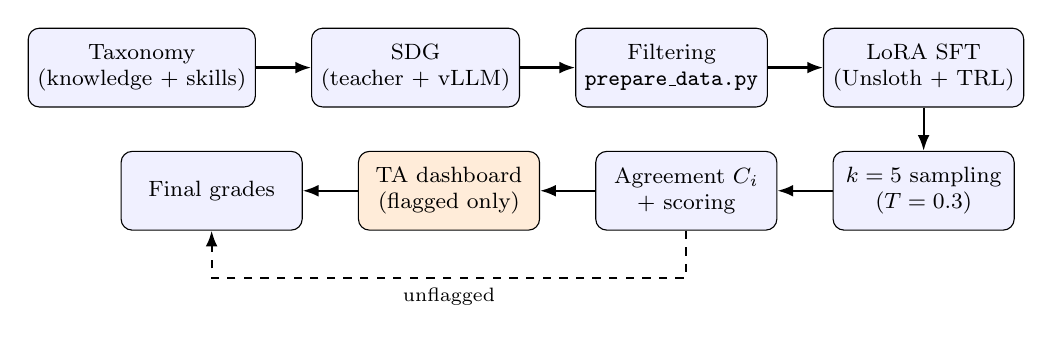
\begin{tikzpicture}[
  node distance=0.55cm and 0.7cm,
  box/.style={draw,rounded corners,align=center,minimum height=1.0cm,minimum width=2.3cm,font=\footnotesize,fill=blue!6},
  hbox/.style={box,fill=orange!15},
  arr/.style={-{Latex[length=2mm]},thick}]
  \node[box] (tax) {Taxonomy\\(knowledge + skills)};
  \node[box,right=of tax] (sdg) {SDG\\(teacher + vLLM)};
  \node[box,right=of sdg] (filt) {Filtering\\\texttt{prepare\_data.py}};
  \node[box,right=of filt] (lora) {LoRA SFT\\(Unsloth + TRL)};
  \node[box,below=of lora] (samp) {$k=5$ sampling\\($T=0.3$)};
  \node[box,left=of samp] (agg) {Agreement $C_i$\\+ scoring};
  \node[hbox,left=of agg] (ta) {TA dashboard\\(flagged only)};
  \node[box,left=of ta] (out) {Final grades};
  \draw[arr] (tax)--(sdg); \draw[arr] (sdg)--(filt); \draw[arr] (filt)--(lora);
  \draw[arr] (lora)--(samp); \draw[arr] (samp)--(agg); \draw[arr] (agg)--(ta);
  \draw[arr] (ta)--(out);
  \draw[arr,dashed] (agg.south) -- ++(0,-0.6) -| node[pos=0.25,below,font=\scriptsize]{unflagged} (out.south);
\end{tikzpicture}
\caption{\gradeai{} pipeline. Orange: human-in-the-loop step.
\todo{}{Replace/refine diagram; add training-vs-inference grouping boxes if desired.}}
\label{fig:pipeline}
\end{figure}

\subsection{Compute Environment}
Experiments run on the \textbf{Fir} cluster (Digital Research Alliance of Canada), allocation \texttt{def-engine14}, using one NVIDIA H100 80\,GB GPU per job (12 CPUs, 128\,GB RAM) under Slurm. Jobs are scripted in \texttt{jobs/generate\_data.sh}, \texttt{jobs/train\_lora.sh}, \texttt{jobs/serve\_model.sh}, and \texttt{jobs/compare\_adapter.sh}
(see \cref{app:slurm}).

\subsection{Knowledge Taxonomy and Source Grounding}\label{sec:taxonomy}
The taxonomy has two branches. \texttt{taxonomy/knowledge/} contains topic entries grounded in David Liu's CSC236 course notes (mathematical induction, recurrences, program correctness, regular languages, DFAs/NFAs), each with seed question--answer pairs in \texttt{qna.yaml}
tied to verified Markdown sources under \texttt{data/sources/csc236/<topic>/}.
\texttt{taxonomy/compositional\_skills/} contains rubric-grading skills:
\texttt{induction\_sums\_and\_identities}, \texttt{induction\_inequalities}, and
\texttt{induction\_divisibility}.
\todo{}{Add number of seed examples per entry (Table~\ref{tab:data}) and licensing note for course notes.}

\subsection{Synthetic Data Generation via Teacher Distillation}\label{sec:sdg}
Seeds are expanded by an InstructLab synthetic data generation pipeline (\texttt{ilab} 0.xx+,\texttt{instructlab-sdg} 0.x.) into diverse questions, student proof variants, and rubric evaluations. The teacher is \todo{}{Teacher model}. Outputs are merged and shuffled with fixed seeds via \texttt{tools/combine\_sdg.py}.
\todo{}{State which teacher was used for the final adapter and why; report teacher temperature and generation counts.}

\begin{table}[t]
\centering
\caption{Training data statistics after SDG and filtering.}
\label{tab:data}
\begin{tabular}{lrrr}
\toprule
Source & Seeds & Generated & After filtering\\
\midrule
Knowledge (induction, recurrences, \ldots) & \ph{XX} & \ph{X,XXX} & \ph{X,XXX}\\
Skill: sums \& identities & \ph{XX} & \ph{X,XXX} & \ph{X,XXX}\\
Skill: inequalities & \ph{XX} & \ph{X,XXX} & \ph{X,XXX}\\
Skill: divisibility & \ph{XX} & \ph{X,XXX} & \ph{X,XXX}\\
\midrule
Total & \ph{XX} & \ph{X,XXX} & \ph{X,XXX}\\
\bottomrule
\end{tabular}
% TODO [Name 3 - Data Lead]: Fill from SDG output / prepare_data.py logs on Fir.
\end{table}

\subsection{Data Filtering and Token Sanitization}\label{sec:filtering}
\texttt{training/prepare\_data.py} does
\todo{}{Report how many examples each filter removed (a small table or one sentence).}

\subsection{LoRA Parameter-Efficient Fine-Tuning}\label{sec:lora}
We fine-tune the base model (\todo{}{Confirm model identifier/size used}) with LoRA using Unsloth and TRL's \texttt{SFTTrainer}.

\todo{}{LoRA exposition}

\subsection{Model Output Schema and Deterministic Scoring}\label{sec:schema}
For each rubric criterion the model returns \todo{}{confirm} and a one-sentence justification; Points are computed in application code via \todo{}{confirm}.
Student text is [xxx] and the prompt instructs the model to treat it as
data, not instructions, as a first defence against prompt injection.


%==============================================================================
\section{Uncertainty Quantification and Human-in-the-Loop Triage}\label{sec:uq}

\subsection{Multi-Run Self-Consistency Sampling}
For every submission we run $x$ independent inference passes at temperature $T=X$,
\todo{}{Numbers.}

\subsection{Agreement Metric}
\todo{}{...}

\subsection{Flagging Rule and Routing Policy}
A submission $x$ is flagged for mandatory TA review if any criterion is uncertain or the output is invalid:
\todo{}{EXAMPLE:}
\begin{equation}\label{eq:flag}
  g(x)=1 \iff \exists\, i:\; C_i<0.8 \;\;\lor\;\; \text{malformed JSON after one retry}.
\end{equation}
Unflagged submissions receive the consensus grade (still subject to TA spot-check at the instructor's discretion); flagged submissions are routed to the dashboard.



\subsection{TA Dashboard and Interaction Model}
The dashboard (\texttt{app/}) shows the student proof beside the rubric, model-assigned levels,
justifications, and confidence for each criterion. TAs confirm or override; all overrides are logged.
\todo{}{Add a screenshot (\texttt{figures/dashboard.png}) and describe override-logging schema.}

% \begin{figure}[t]\centering
%   \includegraphics[width=0.9\linewidth]{figures/dashboard.png}
%   \caption{TA review dashboard.}\label{fig:dashboard}
% \end{figure}

%==============================================================================
\section{Experimental Setup and Benchmarking}\label{sec:setup}

\subsection{Research Questions}
\todo{}{Refine research questions}
\begin{description}[leftmargin=!,labelwidth=1.2cm,itemsep=3pt]
  \item[RQ1] \emph{Criterion-level accuracy.} Does InstructLab fine-tuning outperform the zero-shot base model in per-criterion agreement with expert TA grades? (Target: $\ge 80\%$ agreement.)
  \item[RQ2] \emph{Semantic invariance.} Does \gradeai{} give consistent grades when proofs are reworded without changing mathematical validity? (Target: $\ge 90\%$ consistency.)
  \item[RQ3] \emph{Calibration and triage.} Does \todo{}{question}
  \item[RQ4] \emph{Ablation.} What are the relative contributions of knowledge injection (Phase 1) and compositional-skill fine-tuning (Phase 2)?
\end{description}

\subsection{Synthetic Test Set Construction}\label{sec:testset}
\todo{}{Confirm with SUngmin}
The benchmark of X synthetic student submissions is built \emph{before} training, kept in \todo{}{X}, and never exposed to SDG or training.
Submissions were generated with Claude 3.5 Sonnet / Opus\todo{}{Confirm exact models used and disclose in AI-use statement.} and seeded with common errors: e.g. omitted or incorrect base cases; misstated inductive hypotheses; circular reasoning; incomplete algebra in the inductive step; and flawless proofs.

\subsection{Semantic Paraphrase Robustness Suite}


\subsection{Baselines and Ablation Variants}
(B1) zero-shot base [MODEL]; (B2) few-shot prompted [MODEL]; (V1) knowledge-only LoRA adapter;
(V2) skill-only LoRA adapter; (V3) full \gradeai{} (knowledge + skill).
\todo{}{Confirm which variants were actually trained; drop V2 if not.}

\subsection{Evaluation Metrics}


%==============================================================================
\section{Results and Discussion}\label{sec:results}
\begin{center}\fbox{\parbox{0.92\linewidth}{\small
\textbf{Status note (delete before submission).} Every number in this section is a
\textcolor{blue!70!black}{placeholder or project target}, not a measured result.
}}\end{center}

\subsection{Per-Criterion Grading Accuracy (RQ1)}
\begin{table}[t]
\centering
\caption{Per-criterion accuracy (\%) against human consensus by induction topic.}
\label{tab:rq1}
\begin{tabular}{lcccc}
\toprule
Model & Sums & Inequalities & Divisibility & Overall ($\kappa$)\\
\midrule
Base zero-shot & \ph{63.0} & \ph{59.5} & \ph{61.7} & \ph{61.4} (\ph{0.42})\\
Base few-shot  & \ph{68.2} & \ph{64.0} & \ph{66.1} & \ph{66.1} (\ph{0.50})\\
\textbf{\gradeai{}} & \ph{\textbf{85.0}} & \ph{\textbf{82.1}} & \ph{\textbf{84.0}} & \ph{\textbf{83.7}} (\ph{0.76})\\
\bottomrule
\end{tabular}
% TODO [Name 5 - Evaluation Lead]: Replace with final cluster run metrics from results/stage1_eval.json
% (overall 61.4 / 83.7 / kappa 0.76 are project targets; per-topic and few-shot/kappa cells are invented fillers.)
\end{table}
\todo{}{Discuss: where does \gradeai{} gain most? Per-level confusion matrix? Macro-F1?}

\subsection{Robustness to Semantic Rewording (RQ2)}
\begin{table}[t]
\centering
\caption{Grade consistency (\%) across the five linguistic styles. Each cell is the share of problems whose grade matches the reference style.}
\label{tab:rq2}
\begin{tabular}{lcc}
\toprule
Style & Base zero-shot & \gradeai{}\\
\midrule
Concise formal & \ph{XX} & \ph{XX}\\
Verbose explanatory & \ph{XX} & \ph{XX}\\
Informal conversational & \ph{XX} & \ph{XX}\\
Algebra-heavy & \ph{XX} & \ph{XX}\\
LaTeX math-mode heavy & \ph{XX} & \ph{XX}\\
\midrule
All five agree & \ph{72.0} & \ph{\textbf{91.5}}\\
\bottomrule
\end{tabular}
% TODO [Name 5]: Fill from results/perturbation_eval.json. Targets: base flips ~28%; GradeAI >= 90% consistent.
\end{table}

\subsection{Selective Classification and Triage Efficacy (RQ3)}
\begin{table}[t]
\centering
\caption{Coverage and error concentration under the flagging rule (\cref{eq:flag}).}
\label{tab:rq3}
\begin{tabular}{lccc}
\toprule
Group & \% of submissions & Accuracy (\%) & Share of all errors (\%)\\
\midrule
Unflagged (auto-accepted) & \ph{82} & \ph{94.8} & \ph{33.1}\\
Flagged (TA review) & \ph{18} & \ph{52.1} & \ph{66.9}\\
\bottomrule
\end{tabular}
% TODO [Name 5]: Fill from results/triage_eval.json.
% NOTE: The placeholder numbers (82/94.8 and 18/52.1) imply flagged cases hold ~66.9% of errors,
% NOT >=72%. Either the real run will differ, or the ">=72% of errors" target needs revisiting.
\end{table}
\todo{}{Add a coverage--risk curve (sweep the threshold on $C_i$) as a figure; state the final EC value.}

% \begin{figure}[t]\centering
%   \includegraphics[width=0.7\linewidth]{figures/coverage_risk.pdf}
%   \caption{Selective risk vs.\ coverage.}\label{fig:covrisk}
% \end{figure}

\subsection{Ablation: Knowledge vs.\ Skill Fine-Tuning (RQ4)}
\begin{table}[t]
\centering
\caption{Ablation over adapter configurations.}
\label{tab:rq4}
\begin{tabular}{lccc}
\toprule
Configuration & Accuracy (\%) & $\kappa$ & Rewording consistency (\%)\\
\midrule
Base (zero-shot) & \ph{XX.X} & \ph{0.XX} & \ph{XX.X}\\
+ Knowledge adapter & \ph{XX.X} & \ph{0.XX} & \ph{XX.X}\\
+ Skill adapter & \ph{XX.X} & \ph{0.XX} & \ph{XX.X}\\
+ Combined (\gradeai{}) & \ph{XX.X} & \ph{0.XX} & \ph{XX.X}\\
\bottomrule
\end{tabular}
% TODO [Name 4 - Training Lead]: Fill from jobs/compare_adapter.sh outputs.
\end{table}

\subsection{Qualitative Error Analysis and Failure Modes}
\todo{}{Pull 3--5 concrete failures from results logs (App.~\ref{app:examples}).}
% CLAUDE Suggested categories: algebraic errors hidden by fluent prose; subtle base-case edge cases; over-penalising unconventional but valid reasoning; justification text that contradicts the level

%==============================================================================
\section{Ethical Analysis and Responsible AI Design}\label{sec:ethics}
% TODO [Name 1 + Name 2]: This section is course-critical (CSC398). Aim for ~1 page; tie to course readings.

\subsection{Student Privacy, Data Sovereignty, and FIPPA}


\subsection{Linguistic and Non-Native-Speaker Bias}

\subsection{Over-Reliance and TA Agency}
\gradeai{} is an assistant, not an arbiter: low-confidence cases require human review and justifications make model reasoning auditable.
Risks remain, such as automation bias on unflagged submissions.
\todo{}{Discuss spot-check policy and monitoring for confident-but-wrong cases.}

\subsection{Transparency, Explainability, and Contestability}
Per-criterion levels and one-sentence justifications let students see why partial credit was awarded and support appeals.
\todo{}{Discuss whether students should be told AI assisted grading, and the appeal path.}

\subsection{Statement on AI Use}
\todo{}{Disclose how AI tools were used in research and writing (including synthetic test-set generation and any drafting help) per CSC398 academic-integrity requirements.}

%==============================================================================
\section{Limitations and Threats to Validity}\label{sec:limits}
\begin{itemize}[leftmargin=*,itemsep=2pt]
  \item See ethics document
\end{itemize}
\todo{}{Revise once results are final; add real limitations discovered during experiments. Consult ethics document for more.}

%==============================================================================
\section{Conclusion and Future Work}\label{sec:conclusion}
% TODO [Name 1]: Rewrite after results are in.
We presented a method to use InstructLab-based synthetic data, LoRA fine-tuning, deterministic scoring, and self-consistency-based triage. \todo{}{unslop} Using this method, we built \gradeai{}, a privacy-preserving, human-in-the-loop system for grading undergraduate proofs that combines  \todo{Name 1}{Summarise the actual headline results here (accuracy, invariance, error concentration).}
Future work includes \todo{}{future work}

\section*{Acknowledgments}
We thank \todo{}{Instructor Rutwa Engineer, [mentors], [Digital Research Alliance of Canada (allocation \texttt{def-engine14})], anyone else.}

%==============================================================================
\begin{thebibliography}{99}\small
% TODO [Name 2]: Verify every entry (authors, venue, year, URL) before submission.
% Entries marked "ADD" still need to be filled in from the literature search.


\bibitem{sudalairaj2024lab}
Shivchander Sudalairaj et al.
\newblock LAB: Large-scale alignment for chatbots.
\newblock arXiv:2403.01081, 2024.

\end{thebibliography}
\todo{}{references}
%==============================================================================
\appendix

\section{Prompt Template}\label{app:prompt}
\begin{lstlisting}
QUESTION:
{question}

RUBRIC:
{rubric_json}

<answer>
{student_answer}
</answer>
\end{lstlisting}
\todo{}{replace prompt}

\section{Sample Mathematical Induction Rubric (JSON)}\label{app:rubric}
\todo{Name 3}{Replace this rubric with a real one from taxonomy or \texttt{test\_set/}.}
\begin{lstlisting}
{
    rubric here
}
\end{lstlisting}

\section{Representative Synthetic Proofs and Model Outputs}\label{app:examples}
\todo{Name 5}{Add 2--3 examples: one correct proof, one with a seeded error (e.g.\ circular reasoning), each with human labels and the model's JSON output and $C_i$ values.}

\section{Fir Slurm Batch Scripts}\label{app:slurm}
\todo{Name 4}{Paste final versions of \texttt{jobs/generate\_data.sh} and \texttt{jobs/train\_lora.sh} (remove any secrets/tokens).}
% \lstinputlisting[language=bash,caption={jobs/generate\_data.sh}]{../jobs/generate_data.sh}
% \lstinputlisting[language=bash,caption={jobs/train\_lora.sh}]{../jobs/train_lora.sh}

\end{document}
